% Section 3
% 2021-08-19
% Alessandro Zanatta

\section{Case study}
\label{section:case-study}

The full models of the following examples are freely available on github \cite{CaseStudies}. All tools obtained the same results, the exception being Verifpal's model for the Needham-Schroeder-Lowe Public Key protocol.

\subsection{Diffie-Hellman key exchange}

We will examine three different models for the Diffie-Hellman key exchange protocol: anonymous, ephemeral and ephemeral with post-compromise of keys. This allows us to explore many advanced features and modelling techniques of each tool. \Cref{fig:dh-key-exchange} shows a schematic representation of the protocol.

In the anonymous version we model an un-authenticated Diffie-Hellman, where no security property can hold as the adversary is free to perform a man-in-the-middle attack \cite{MITM-DH}.

In the ephemeral version we model a client-server Diffie-Hellman exchange in which the server's half key is authenticated (e.g. by an X.509 certificate). The server is willing to execute the protocol with any client, but the server is always authenticated.

Finally, we model a Diffie-Hellman with post-compromise of ephemeral keys. This is how Perfect Forward Secrecy \cite{PFS} is usually tested in the symbolic model. Of course, secrecy of the exchanged messages will not hold.

\begin{figure}[t]
    \setmscoptions
    \begin{msc}{}
        \setmscscale{.7}

        \declinst{client}{}{Client}
        \declinst{server}{}{Server}

        \action*{\parbox{3.5cm}{\centering
                Knows $g, p$\\
                $c \in \Z$\\
                $g_c := \modexp{g}{c}{p}$
            }}{client}

        \nextlevel[5]
        \mess{$g_c$}{client}{server}
        \nextlevel

        \action*{\parbox{3.5cm}{\centering
                Knows $g, p$\\
                $s \in \Z$\\
                $g_s := \modexp{g}{s}{p}$\\
                $\skey{c} := \modexp{g_c}{s}{p}$
            }}{server}

        \nextlevel[6]
        \mess{$g_s$}{server}{client}
        \nextlevel

        \action*{\parbox{3.5cm}{\centering
                $\key{cs} := \modexp{g_s}{c}{p}$
            }}{client}
        \nextlevel

    \end{msc}
    \centering
    \caption{Diffie-Hellman key exchange protocol}
    \label{fig:dh-key-exchange}
\end{figure}

\subsubsection{Implementation notes}

We will describe implementation details worth of note in the next paragraphs. Notice that we will use an incremental approach, describing only what was \textit{changed} between different versions.

\paragraph{Anonymous} The implementation of the anonymous version is straightforward. We use two particular constructs for Proverif and Tamarin to store keys: tables and persistent facts, respectively. Both serve the same purpose: store some permanent information (which is not, by default, available to the attacker). The first supports two operations: \textit{insert} and \textit{get}. The latter is, in essence, a \textit{fact} with the additional property of never being removed from the global state.

\paragraph{Ephemeral} In this version, the server half key needs to be authenticated\footnote{An additional requirement is that, while the half key cannot be mutated by the attacker, it must be available to it.}. In Verifpal there is a single (simple) way: guarded variables. Guarded variables (variables between square brackets) are not mutable by the attacker (but known by it). In Tamarin we model this with a simple private channel ruled by a passive attacker. This is done with the following multiset rewriting rule:


\lstset{language=tamarin}
\begin{lstlisting}
rule CertificateExchange:
    [ CertificateOut(x) ] --> [ CertificateIn(x), Out(x) ]
\end{lstlisting}

Finally, in Proverif we model this with a table, additionally making sure to output everything we insert into it. We could have also used a private channel, but that makes the verification of certain queries yield an inconclusive result.

\paragraph{Post-compromise} In Tamarin, we define the following rule (for both client and server):

\lstset{language=tamarin}
\begin{lstlisting}
rule RevealClientEphemeralKey:
    [ ClientEphemeralKey(c) ]
  --[ RevealedClientEphemeralKey(c) ]->
    [ Out(c) ]
\end{lstlisting}

This actually models a \textit{generic} compromise rule. We can exploit timepoints in security properties to assert that the compromise must happen \textbf{after} some other event (e.g. parties has exchanged a message), making this a post-compromise.

In Proverif, we define a process macro which simply outputs the ephemeral key in phase 1:

\lstset{language=proverif}
\begin{lstlisting}
let PostRevealClientEphemeralKey =
    phase 1;

    (* Get the client's ephemeral key and output it *)
    get ClientEphemeralKeyTable(c) in
    out(io, c);
    event PostRevealedClientEphemeralKeyTable(c);
    0.
\end{lstlisting}

\lstset{language=verifpal}
Modeling post-compromise in Verifpal requires using phases again. We can then use Verifpal's built-in construct for revealing terms: \lstinline{leaks x}.
\newpage
\begin{lstlisting}
phase [1]

principal Client [
    leaks c
]

principal Server [
    leaks s
]
\end{lstlisting}

\subsection{Needham-Schroeder Public Key protocol}
\label{sec:NSPK}

\begin{figure}[t]
    \setmscoptions
    \begin{msc}{}
        \setmscscale{.7}

        \declinst{alice}{}{Alice}
        \declinst{bob}{}{Bob}

        \action*{\parbox{3.5cm}{\centering
                Knows $\skey{A}, \pkey{A}$\\
                Knows $\pkey{B}$
            }}{alice}

        \action*{\parbox{3.5cm}{\centering
                Knows $\skey{B}, \pkey{B}$\\
                Knows $\pkey{A}$
            }}{bob}
        \nextlevel[4]

        \action*{\parbox{3.5cm}{\centering
                Generates $N_A$
            }}{alice}

        \nextlevel[3]
        \mess{$\enc{N_A, A}{\pkey{B}}$}{alice}{bob}
        \nextlevel


        \action*{\parbox{3.5cm}{\centering
                Generates $N_B$
            }}{bob}

        \nextlevel[3]
        \mess{$\enc{N_A, N_B}{\pkey{A}}$}{bob}{alice}
        \nextlevel[2]
        \mess{$\enc{N_B}{\pkey{B}}$}{alice}{bob}

    \end{msc}

    \centering
    \caption{Simplified Needham-Schroeder Public Key protocol}
    \label{fig:NSPK}
\end{figure}

The next case-study is the Needham-Schroeder Public Key protocol. Two versions are considered: the flawed version and the fixed one (by Lowe \cite{NSPK_LoweGavin}). A schematic representation of the flawed protocol is shown in \cref{fig:NSPK}, which assumes that clients already know each other's public keys. In the fixed version, message 2 is changed from $\enc{N_A, N_B}{\pkey{A}}$ to $\enc{B, N_A, N_B}{\pkey{A}}$.

\subsubsection{Implementation notes}

In order to re-discover the attack, we model the protocol in a way that allows the attacker to decide whom the honest initiator executes the protocol with. The responder, however, only wishes to engage with the honest initiator.

\newpage
\paragraph{Flawed}

In Proverif, to allow the behaviour described above, we let the attacker send the principals to the initiator at the start of its macro:

\lstset{language=proverif}
\begin{lstlisting}
let Initiator() =
(* Attacker sends communicating parties *)
in(io, (X: Principal, rUser: Principal));

(* We restrict them: X must be honest and they must be different *)
let iUser = isHonest(X, Alice, Bob) in
if iUser <> rUser then (* Protocol starts here *)
\end{lstlisting}

In Tamarin we follow a very similar approach, but we define the initiator to be always Alice (i.e. the attacker chooses \textit{only} the responder). Using the same strategy of Proverif would lead to a very complex protocol with termination issues.

In Verifpal the implementation is straightforward, with a single caveat: when pre-sharing public keys we need to guard only Alice key. This allows the attacker to mutate Bob's key to its own.

\lstset{language=verifpal}
\begin{lstlisting} 
Alice -> Bob: [K_PA]
Bob -> Alice: K_PB
\end{lstlisting}


\paragraph{Fixed} No changes to the models were applied but the fix to the Needham-Schroeder Public Key protocol described at the start of \cref{sec:NSPK}.

\subsection{Results}
\begin{figure}[t]
    \centering
    \makebox[\textwidth][c]{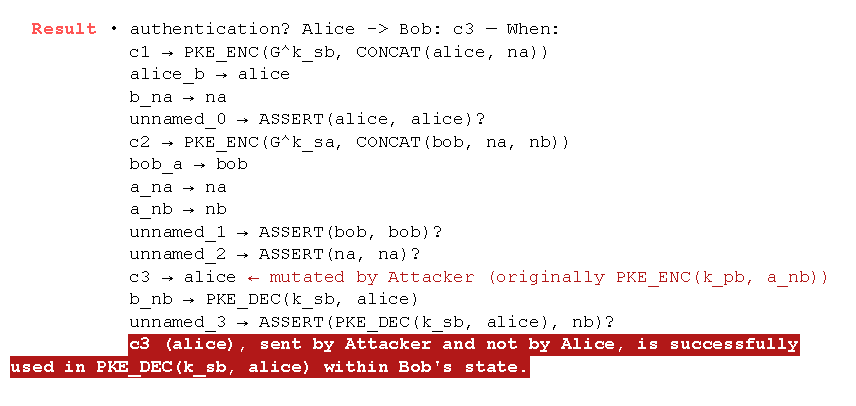
\includegraphics{verifpal-nspk-trace}}
    \caption{Verifpal fixed NSPK attack trace.}
    \label{fig:verifpal-nspk-trace}
\end{figure}

All three tools returned the expected result:
\begin{itemize}
    \item{Diffie-Hellman
                \begin{itemize}
                    \item Anonymous: secrecy and authentication of both parties do not hold;
                    \item Ephemeral: secrecy of client messages and authentication of the server hold. Secrecy of server messages does not hold as the server is willing to initiate a run of the protocol with anybody, even the attacker;
                    \item Post-Compromise Ephemeral: secrecy of client messages no longer holds, but messages from the server are still authenticated.
                \end{itemize}
          }
    \item{Needham-Schroeder Public Key
                \begin{itemize}
                    \item Flawed: Secrecy of the nonces and authentication do not hold.
                    \item Fixed: Nonce secrecy and authentication of the initiator hold. However, as the initiator is willing to execute the protocol with anyone, authentication of the responder does not hold.
                \end{itemize}
          }
\end{itemize}

\lstset{language=verifpal}
There is an exception: Verifpal reports the fixed Needham-Schroeder Public Key  protocol as flawed and finds attack traces for both authentication and confidentiality queries.
Inspecting the result shown in \cref{fig:verifpal-nspk-trace} carefully we can notice a strange result: in the penultimate line, the checked primitive \lstinline{ASSERT}\footnote{A checked primitive in Verifpal is a primitive that aborts execution of the protocol run when it fails. A question mark at the end of a primitive indicates that it is checked. The \lstinline{ASSERT} primitive simply checks that both arguments are actually the same term.} fails right after. In reality, an execution with a failed assertion should be immediately aborted, but Verifpal uses such executions to falsify queries.

Moreover, \textbf{this is not a bug} but the intended behaviour. In a mail on the Verifpal's mailing list we can find the Verifpal's author opinion on a similar problem: ``This analysis result appears to be completely correct to me. The ASSERT call occurs after Bob decrypts enca. So yes, the protocol does not finish its run, but Bob still manages to use the non-authentic enca before the protocol is aborted! Hence the result'' \cite{VerifpalMail}.

It does not seem like there is a way of changing this behaviour, but we can indeed confirm that Verifpal is reporting false traces by looking at the penultimate line: if it contains a checked primitive that obviously fails, then the attack trace is incorrect, otherwise there may be an attack. Notice that this does not mean that there is no attack trace for a certain property as the incorrect one might be masquerading a valid one.